\documentclass[british]{amsart} \usepackage{lmodern}

% Bibliography
\usepackage[backend=biber,style=alphabetic]{biblatex} 
\addbibresource{spt.bib}
%\usepackage[style=alphabetic]{biblatex} 
%\addbibresource{spt.bib}

\renewcommand{\sfdefault}{lmss} \renewcommand{\ttdefault}{lmtt}
\usepackage[T1]{fontenc} \usepackage[latin9]{inputenc} \usepackage{verbatim}
\usepackage{amstext} \usepackage{amsthm} \usepackage{amssymb}
\usepackage{subfiles}
\usepackage{graphicx}

\makeatletter
%%%%%%%%%%%%%%%%%%%%%%%%%%%%%% Textclass specific LaTeX commands.
\numberwithin{equation}{section} \numberwithin{figure}{section}
\theoremstyle{plain} \newtheorem{thm}{\protect\theoremname}[section]
\theoremstyle{definition} \newtheorem{defn}[thm]{\protect\definitionname}
\theoremstyle{plain} \newtheorem{assumption}[thm]{\protect\assumptionname}
\theoremstyle{plain} \newtheorem{lem}[thm]{\protect\lemmaname}
\theoremstyle{plain} \newtheorem{prop}[thm]{\protect\propositionname}
\theoremstyle{remark} \newtheorem{rem}[thm]{\protect\remarkname}
\theoremstyle{plain} \newtheorem{cor}[thm]{\protect\corollaryname}

%%%%%%%%%%%%%%%%%%%%%%%%%%%%%% User specified LaTeX commands.
\usepackage{color} \usepackage[colorlinks=true,linkcolor={blue}]{hyperref}

\usepackage{amsfonts}
%\renewenvironment{lyxgreyedout}{\color{red}\bgroup}{\egroup}

\makeatother

\usepackage[british]{babel} \usepackage[babel]{csquotes}
\addto\captionsbritish{\renewcommand{\assumptionname}{Assumption}}
\addto\captionsbritish{\renewcommand{\definitionname}{Definition}}
\addto\captionsbritish{\renewcommand{\lemmaname}{Lemma}}
\addto\captionsbritish{\renewcommand{\propositionname}{Proposition}}
\addto\captionsbritish{\renewcommand{\remarkname}{Remark}}
\addto\captionsbritish{\renewcommand{\theoremname}{Theorem}}
\addto\captionsenglish{\renewcommand{\assumptionname}{Assumption}}
\addto\captionsenglish{\renewcommand{\definitionname}{Definition}}
\addto\captionsenglish{\renewcommand{\lemmaname}{Lemma}}
\addto\captionsenglish{\renewcommand{\propositionname}{Proposition}}
\addto\captionsenglish{\renewcommand{\remarkname}{Remark}}
\addto\captionsenglish{\renewcommand{\theoremname}{Theorem}}
\addto\captionsenglish{\renewcommand{\corollaryname}{Corollary}}
\providecommand{\assumptionname}{Assumption}
\providecommand{\definitionname}{Definition} \providecommand{\lemmaname}{Lemma}
\providecommand{\propositionname}{Proposition}
\providecommand{\remarkname}{Remark} \providecommand{\theoremname}{Theorem}
\providecommand{\corollaryname}{Corollary}

%%%%%%%%%%%%%%%%%%%
\renewcommand{\d}[1]{\mathop{\mathrm{d}{#1}}}
\newcommand{\msquared}{\mathcal{M}^{2}_{0,T}}
\newcommand{\realnumbers}{\mathbb{R}} \newcommand{\ranget}{t\in[0,\infty)}
\newcommand{\filtration}[1]{\mathcal{F}_{#1}}
\newcommand{\defeq}{\mathop{\triangleq}} \newcommand{\almostsurely}{\text{a.s.}}
\newcommand{\abs}[1]{\mathop{|{#1}|}} \newcommand{\market}{\mathcal{M}}
\newcommand{\rangei}{i=1,\dots,n} \newcommand{\measure}{\mathbb{P}}
\newcommand{\probabilityspace}{(\Omega,\filtration,\measure)}
\newcommand{\E}[1]{\mathbb{#1}} \newcommand{\valueprocess}[2]{V^{#1}(#2)}
\newcommand{\norm}[1]{\left\lVert#1\right\rVert}
\newcommand{\V}{V^{w,\pi}}
\newcommand{\Vmu}{V^{\mu}}
%%%%%%%%%%%%%%%%%%%

\begin{document}
\title{Functionally Generated Portfolios in Stochastic Portfolio Theory}
\author{Lawrence Edwards} \maketitle

\newpage

\tableofcontents{}

\newpage

%\section{Introduction} \include{introduction} \section{Preliminaries}

%%%%%%%%%%%%%%%%%%%%%%%%%%%%%%%%%%%%%%%%%%%%%%%%%%%%%%%%%%%%%%%%%%%%
\section{Introduction}

Stochastic Portfolio Theory (SPT) is a mathematical theory of how portfolios of
risky assets evolve over time. Unlike Modern Portfolio Theory (MPT) and Capital
Asset Pricing Model (CAPM) theories, SPT is descriptive as opposed to normative
and is therefore consistent with empirical observations of the market.

SPT models prices of assets using continuous semi-martingales. By convention the
theory uses the logarithmic representation of prices and therefore refers to the
growth rates of assets and portfolios. In this context, the logarithmic
representation allows us to apply the tools of stochastic calculus in a more
convenient manner. 

The theory is often presented referring to non-dividend paying stocks for
reasons of simplicity, but the theory has been shown to be compatible with
dividend paying stocks and is applicable to other classes of assets.
Additionally processes with discontinuities, such as jumps have been
incorporated into the theory. The convention is to assume the stocks have a
single share outstanding, so that the prices reflect the total market
capitalisation of the stock.

The theory builds on the concept of \textit{investment strategies}, which are
defined as progressively measurable processes that represent the proportion of
the total wealth invested in each stock at a particular time.
\textit{Portfolios} are defined similarly to investment strategies, but 
the weights represent the fraction of wealth invested in a particular stock at
any point in time, and are always fully invested in the market. The theory
presents a formula for the (always positive) value process of a strategy,
defined using the sum of the weighted logarithmic returns of a strategy plus a
process, called the \textit{excess growth rate process}, which forms a
fundamental tool in examining how arbitrage opportunities can arise.

An important portfolio, called the \textit{market portfolio} is defined, where
the investment strategy is to hold a fraction of wealth corresponding to a
stocks relative capitalisation. The excess growth rate of this portfolio is
interpreted as the market's intrinsic volatility which is shown to lead to
arbitrage opportunities relative to the market when sufficiency (boundedness
away from zero) conditions are met.

The theory examines \textit{relative arbitrage} relationships between investment
strategies, both in a \textit{strong arbitrage} and \textit{weak arbitrage}
form. In a link with the Benchmark approach to Mathematical finance
\cite{platen2006}, SPT defines a \textit{numeraire property} of a strategy,
which can be shown to preclude arbitrage over any time horizon.

The cornerstones of SPT are \textit{functionally generated portfolios}, and
Fernholz's Master Equation. Functionally generated portfolios are
portfolios generated by $\mathcal{C}^2$ \textit{generating functions} that allow
for the formulaic construction of well-performing portfolios that
do not require estimation of the drifts or volatilities of the stocks. The
primary machinery of SPT in which all relative arbitrages are
constructed, called the \textit{Master Equation} measures the performance of any
portfolio relative to the market portfolio. This performance is decomposed into
a stochastic part of infinite variation (written as a function of the market
weights), plus a finite variation component. By choosing a suitable generating
function the stochastic term can be bounded from below, producing relative
arbitrage opportunities.

Some generalisations of functionally generated portfolios have recently been
proposed, e.g. Strong et. al. \cite{strong2014generalizations} demonstrate
how the generating function may be dependent on other sources of information,
such as sentiment or other market factors. Pal and Wong \cite{pal2013} prove
that subject to the class of portfolios being only those generated by current
market capitalisations, then a slight generalisation of functionally generated
portfolios are the only class of portfolios that permit relative arbitrage.

Several such classes, corresponding to different assumptions on market
behaviour, have been introduced and studied in SPT; these are:

\begin{itemize}

\item \textbf{Diverse:} SPT introduces a definition of diversity as being the
condition that the market weight processes weights are bounded from above by a
number smaller than one, effectively meaning that no single company can dominate
the entire market capitalisation.

Diversity is clearly observed in real markets, and its validity is virtually
guaranteed in mature markets by anti-trust regulations. This assumption was
first studied in detail using the tools of SPT by Fernholz, Karatzas and
Kardaras \cite{fernholz2005}, who introduced formal definitions of diversity and
proved that under an additional \textit{non-degeneracy} condition on the stock
volatilities, relative arbitrages exist in such markets - both over sufficiently
long time horizons and as well as over arbitrarily short time horizons.

\item \textbf{Intrinsically Volatile:} The condition of "sufficiently intrinsic
volatility" requires the excess growth rate of the market portfolio to be
bounded away from zero.

Fernholz in \cite{fernholz2002} argued that this condition holds for real
markets, and without any additional assumptions, showed that there exists
relative arbitrage over sufficiently \textit{long} time horizons, where the
duration required to achieve the relative arbitrage depends on the magnitude of
the lower bound for average market volatility (see also
\cite{fernholz2005relative}.

It remains an open problem whether a relative arbitrage over arbitrarily
\textit{short} time horizons exists. Short horizon arbitrage  has been shown to
exist in volatility-stabilised markets (\cite{banner2008short} generalised
volatility-stabilised markets (\cite{pickova2014generalized}), and Markovian
intrinsically volatile models (Proposition 2 of \cite{fernholz2009}).

\item \textbf{Rank-based:} In Rank-based methods, the drift and volatility
processes of each stock are made to depend on the stocks rank according to its
capitalisation.

Fernholz first introduced a framework for studying the performance of portfolios
which put weights on stocks based on their rank instead of their name, allowing
him to explain certain phenomena observed in real markets in
\cite{fernholz2002}. These models were introduced based on the observation that
the distribution of capital according to rank by capitalisation has been very
stable over the past decades. The dynamics of stocks in these models have been
studied extensively, but the question of existence of (asymptotic) relative
arbitrage has not been addressed yet. A very simple case of a rank-based model,
the Atlas model, was introduced and studied in \cite{banner2005atlas} and
\cite{ichiba2011hybrid}.

\end{itemize}

In this dissertation, we aim to provide a detailed introduction to the theory
and proofs of SPT, leading to the proof of the Master Equation. Using this as a
foundation we examine the diverse model and show how relative arbitrage
opportunities are created, as well as identifying all of the relevant
assumptions and conditions required for these arbitrages.

Once armed with this theory we then examine various simulations of these
strategies using a proprietary dataset and commercial backtesting framework to
see how these portfolios would perform under real conditions taking into account
trading costs and market impact.

% TODO: Expand introduction with details on simulation
% We carry out an empirical study of the constructed portfolios in Section
%6, demonstrating that our adjustments of the diversity-weighted portfolio would
%have outperformed quite considerably the S&P 500 index, if imple- mented on the
%index constituents over the 25 year period between January 1, 1990 and December
%31, 2014. In this study we incorporate 0.5% proportional transaction costs,
%delistings due to bankruptcies, mergers and acquisitions, and distributions such
%as dividends. We compute the relative returns of our portfolios over this
%period, as well as the Sharpe ratios relative to the market index. We discuss
%the results and possible future work in Section 7.

%%%%%%%%%%%%% END INTRODUCTION %%%%%%%%%%%%%%%%%%%%%%%%%
\newpage
\section{Preliminaries}

This chapter reviews some results and definitions from and fixes notation for
the remainder of the paper.

\subsection{Log-Returns}

We define the daily log-return of a stock price as the daily increment
of the natural logarithm of this price. If $X(t)$ represents the stock
price at time $t$, then the log-return $R(t)$ is defined as

\begin{equation}
  R(t) 
    \defeq \log{X(t+\Delta t)} - \log{X(t)} 
    = \log \left( \frac{\log{X(t+\Delta t)}}{\log{X(t)}} \right),
  \quad \ranget.
\end{equation}

% TODO: Definitions: Add geometric vs arithmetic return

\subsection{Probability and Stochastic Processes}

This section provides a concise overview of stochastic calculus for
diffusion processes. The model for continuous stock prices presented
here has an extensive literature can be found in \cite{shreve1991}.

Throughout, we work on a filtered probability space denoted
by $(\Omega,\mathcal{F},\left\{ \mathcal{F}_{t}\right\} _{t\ge0},P)$
where:

\begin{itemize}
  \item $\Omega$ denotes the space of all events,
  \item $\mathcal{F}$ denotes the set of all measurable events,
  \item $\{ \mathcal{F}_{t}\}_{t\ge0}$ denotes the filtration
        - a family of $\sigma$-algebras contained in $\mathcal{F}$ with
        the property that if $s<t$ then $\mathcal{F}_{s}\subset\mathcal{F}_{t}$. 
\end{itemize}

\begin{defn} [Stochastic Processes]
  The modelling of random assets is based on stochastic processes, which are
  families $X(t)$  of random variables $X(t):\Omega\to\mathbb{R}$ for $t\in[0,T]$,
  where $X(0)$ is constant.
\end{defn}

\begin{defn} [Brownian Motion]
  A Standard Brownian motion $W$ is a stochastic process which
  is a mapping $W:[0,\infty)\times\Omega\to\mathbb{R}$ for a probability
  space $(\Omega,\mathcal{F},P)$ which has the properties:

  \begin{enumerate}
    \item $W(0)=0$, a.s.,
    \item $W(t)$ has independent increments,
    \item $W(t)$ has stationary increments $W(t)-W(s)\thicksim\mathcal{N}(0,t-s)$
          for $0\le s<t<\infty,$
    \item the sample trajectories for almost all $\omega\in\Omega$ the paths
          $t\to W(t,\omega)$ are almost surely continuous.
  \end{enumerate}
\end{defn}

\subsection{Ito Calculus}

We briefly introduce Ito calculus, beginning with definition of a simple process
and the Ito integral for simple functions, and then move to the more general
definition of the Ito integrals. Square-integrable (random) adapted processes,
introducing the notion of measureability. 


\begin{defn}
  A stochastic process is called $\mathcal{F}_{t}$-\textbf{measurable} if 

  \begin{equation}
    X^{-1}(B)=\left\{ \omega\in\Omega:X(\omega)\in B\right\} \in\mathcal{F},\;\;\text{for every Borel set }B\in\mathcal{B}(\mathbb{R}).
  \end{equation}

  the knowledge of $X$ depends only on the information known up until time $t$.
\end{defn}
%
\begin{defn}
The \textbf{filtration} generated by a stochastic process $X(t)$
is a family of $\sigma$-fields is defined as, 
\[
\mathcal{F}^{X}(t)\triangleq\sigma\left\{ X(s);0\le s\le t\right\} ,\;\;\forall t\in[0,T].
\]
\end{defn}
%
\begin{defn}
A process $\left\{ X(t),\mathcal{F}_{t},t\in[0,T]\right\} $ is \textbf{adapted}
to a filtration $\mathcal{F}$ if $X(t)$ is $\mathcal{F}_{t}$-measurable
for all $t\in[0,T]$. 
\end{defn}
%
\begin{defn}
Let $f(t),t\ge0$ be a stochastic process with a.s. continuous paths
adapted to the filtration $\mathcal{F}_{t}=\mathcal{F}^{W}(t)$, then
we define the $\mathcal{M}^{2}$ space of processes as
\[
\mathcal{M}^{2}\triangleq\left\{ f:[0,T]\times\Omega\to\mathbb{R}:f\,\text{is\,adapted},\,\mathbb{E}\left(\int_{0}^{T}f^{2}(t)dt\right)<\infty\right\} .
\]
\end{defn}
%
\begin{defn}
A process $f\in\mathcal{M}^{2}$ is \textbf{simple} if we can find
a partition $0=t_{0}<t_{1}<...<t_{n}=T$, and $\mathcal{F}_{t_{k}}$-measurable
random variables $\xi_{k}$ with $\mathbb{E}(\xi_{k}^{2})<\infty$,
$k=0,1,...,n-1$ such that
\[
f(t,\omega)=\xi_{0}(\omega)\mathbf{1}_{\{0\}}(t)+\sum_{k=0}^{n-1}\xi_{k}(\omega)\mathbf{1}_{(t_{k},t_{k+1}]}(t),
\]
 and we write $f\in\mathcal{S}^{2}$ to denote the class of all simple
processes.
\end{defn}
%
\begin{defn}
\textbf{The Ito integral} of a stochastic process $X(t)$ on a partition
$[0,T]$, $0=t_{0}<t_{1}<\ldots<t_{n}=T$, with respect to the Brownian
motion $W$ given by
\[
\int_{0}^{T}X(t)dW(t)\triangleq\lim_{n\to\infty}\sum_{j=0}^{n-1}X(t_{j})\left(W(t_{j+1})-W(t_{j})\right).
\]
%
\end{defn}
Let $X(t)$ be a generalised Brownian motion process or an Ito process.
That is, let $X(t)$ have the following dynamics
%
\begin{equation}
dX(t)=a(t,X(t))dt+b(t,X(t))dW(t),
\end{equation}

where $W(t)$ is a standard Brownian motion process.

Let $F(t,X(t))$ be a function with continuous second derivatives,
where $F$ and $X$ have a functional dependence. Then $F(t,X(t))$
is also an Ito process and has the following dynamics

\begin{align*}
dF(t, & X(t))=\frac{\partial F}{\partial t}(t,x)dt+\frac{\partial F}{\partial x}(t,x)dX(t)+\frac{1}{2}\frac{\partial^{2}F}{dx^{2}}(t,x)(dX(t))^{2}\\
= & \left(\frac{\partial F}{\partial t}(t,x)+a(t,x)\frac{\partial F}{\partial x}(t,x)+\frac{1}{2}b^{2}(t,x)\frac{\partial^{2}F}{\partial x^{2}}(t,x)\right)dt+b(t,x)\frac{\partial F}{\partial x}(t,x)dW(t).\\
\end{align*}

% TODO: Definitions: Define progressively measurable process

\begin{thm} [Multidimensional Ito formula]

  For a $n$-dimensional Ito process $X_{i}(\cdot)$ with $d$ independent Brownian motions and a
  matrix $[\beta_{ij}(t)]$, $i=1,\dots,n$ and $\nu=1,\dots,d$ of $\mathcal{L}_{[0,T]}^{2}$ processes

  \begin{equation}
    \d{X_{i}(t)} = \alpha_i(t) + \sum_{\nu=1}^d \beta_{i\nu}(t)\d{W_{\nu}(t)}
    \quad i=1,\dots,k,
  \end{equation}

  then for a given function $F:[0,\infty) \times \mathbf{R}^d \to \mathbf{R}$, of
  class $\mathcal{C}^2$ in the first variable and $\mathcal{C}^1$ in the others
  and write $Y(t)=F(t,X(t))$. Then $Y$ is an Ito process with

   \begin{gather}
    \begin{split}
    \d{Y(t)} &= F_{t}(t, X(t))\d{t} + \sum_{i=1}^n F_{x_{i}}(t,X(t)) \alpha_{i}(t)\d{t} \\
             & + \sum_{i=1}^n F_{x_{i}}(t,X(t)) \sum_{\nu=1}^n \beta_{i\nu}(t)\d{W_{\nu}(t)} \\
             & + \frac{1}{2} \sum_{\nu=1}^d \sum_{i=1}^n \sum_{j=1}^n
                  F_{x_{i}x_{j}}(t,X(t)) \beta_{i\nu}(t) \beta_{j\nu}(t)\d{t}.
    \end{split}
  \end{gather}

  Where we are interested in only the dynamics of a single Ito process
  $X_{i}(\cdot)$ for a specific $i$, with $d$-dimensional Brownian motion, this
  can be written for $\rangei$, as

  \begin{gather}
    \begin{split}
    \d{Y(t)} &= F_{t}(t, X(t))\d{t} + F_{x}(t,X(t)) \alpha_{i}(t)\d{t} \\
             & + F_{x}(t,X(t)) \beta_{ij}(t)\d{W_{j}(t)} \\
             & + \frac{1}{2} \sum_{\nu=1}^d F_{xx}(t,X(t))
                \beta_{i\nu}(t) \beta_{j\nu}(t)\d{t},\\
    \end{split}
  \end{gather}


\end{thm}

\newpage

\section{Stochastic Portfolio Theory}

%%%%%%%%%%%%%%%%%%%%%%%%%%%%%%%%%%%%%%%%%%%%%%%%%%%%%%%%%%%%%%%%%%%%
\subsection{The Market Model}

We introduce the market model introduced by Fernholz (\cite{fernholz1999pgf} and
later in \cite{fernholz2009}) of stock price processes represented by continuous
semimartingales, which is fairly standard in continuous-time financial theory
and investigated in detail in \cite{karatzas1998}.

A number of assumptions are made for clarity of expression, amongst these are:

\begin{itemize}
  \item the number of companies in the market is fixed, and companies do not 
        break up or merge,
  \item the number of shares of a company remains constant,
  \item trading is in continuous time,
  \item dividends are paid continuously,
  \item there are no transaction costs or taxes,
  \item fractional ownership of shares are allowed.
\end{itemize}

Although these assumptions are not based on the empirical facts of the market,
they are made to improve the clarity and simplicity of the exposition of the
theory. In most cases the theory can be generalised to include them. An
additional convention in SPT we adopt is to assume that each company has a
single share outstanding, so that the price of the stock is equivalent to it's
market capitalisation.

Our setting is a market $\market$, with $n$ stocks, and $d$-dimensional
independent Brownian motion $W(\cdot)$ (with $d \ge n$), defined on a
probability space $\probabilityspace$ as

\begin{gather}
  \label{eq:marketmodel}
  \begin{split}
    \d{B(t)} &= B(t)r(t)\d{t},  
      \quad \ranget, \\
    \d{X_{i}(t)} &= 
          X_{i}(t) 
          \left(
              b_{i}(t)dt + \sum_{\nu=1}^{d} \sigma_{i\nu}(t) dW_{\nu}(t)
          \right),
      \quad \rangei,
      \quad \ranget
  \end{split}
\end{gather}

where $W = \left\{ W(t)=(W_{1}(t),...,W_{d}(t)),\filtration{t},\ranget \right\}$
are the independent $d$-dimensional Brownian motions, $r(\cdot)$ is the
interest-rate process for the money-market, $B(0)=1$. The price process
$X_{i}(t)$ represents the price of the $i$th stock, where $X_{i}(0) = x_{i} > 0$
are the (strictly positive) initial values of the stock prices.

We also assume the $\filtration{}$-progressively measurable $(n \times 1)$
process $b(\cdot)$ called the \textit{rates of return}, and the $(n \times d)$
process $\sigma_{i\nu}(t)$ of \textit{volatilities} satisfy the integrability
conditions: 

\begin{equation*}
  \int_{0}^{T} 
  \abs{r(t)} 
  \d{t} +
  \sum_{i=1}^{n} \int_{0}^{T} 
    \left( 
        \abs{b_{i}(t)} +
        \sum_{\nu=1}^{d} ( \sigma_{i\nu}(t)^2  ) 
        \right) \d{t} < \infty,
  \quad T \in [0, \infty),
  \quad \almostsurely.
  \end{equation*}


The stock price process (\ref{eq:marketmodel}) can be written using the notation 

\begin{equation}
  \label{eq:stockpriceprocessdiff}
    \frac{\d{X_{i}(t)}}{X_{i}(t)} = b_{i}(t)\d{t} + \sum_{\nu=1}^{d} \sigma_{i\nu}(t) dW_{\nu}(t),
  \quad \rangei
  \quad \ranget,
\end{equation}

where the first ratio defined as

\begin{equation*}
  \frac{\d{X_{i}(t)}}{X_{i}(t)} \defeq 
  \int_{0}^{t} b_{i}(s)\d{s} + 
  \int_{0}^{t} \sum_{\nu=1}^{d} \sigma_{i\nu}(s) dW_{\nu}(s),
  \quad \rangei,
\end{equation*}

is referred to as the \textit{instantaneous} return on the stock.

We now introduce the formal definition of a market (\market) by 

\begin{defn} 
[
  {\cite[Definition 2.2]{fernholz1999pgf}}
]
\label{def:market}

A market is a family $\market = \{X_{i},\dots,X_{n}\}$ of stocks, defined as in
(\ref{eq:marketmodel}), for which there is a number $\epsilon>0$ such that

\begin{equation}
  \label{eq:strongnondegeneracy}
  x \sigma(t) x^{T} \ge \epsilon \|x\|^{2}, 
  \quad x \in \mathbf{R}^{n}, 
  \quad \ranget,
  \quad \almostsurely.
\end{equation}

Here, $\sigma(t) = \{\sigma_{i\nu}(t)\}$ where $\rangei$ and $\nu=1,\dots,d$ is the
covariance matrix defined in (\ref{eq:marketmodel}) and $T$ denotes
transposition.

\end{defn}

The \textit{strong nondegeneracy} condition (\ref{eq:strongnondegeneracy}) is a 
common condition regarding market volatility, sometimes known as \textit{strict
nondegeneracy}, and can be found, for example, in \cite{shreve1991}. It 
expresses the requirement that the eigenvalues of the market covariation 
matrix be bounded away from zero. 

%%%%%%%%%%%%%%%%%%%%%%%%%%%%%%%%%%%%%%%%%%%%%%%%%%%%%%%%%%%%%%%%%%%%
\subsubsection{Stocks}

We follow the convention used by Fernholz and use a logarithmic representation
for stocks.

The logarithmic return (log return) of a financial asset is the change in the
natural logarithm of the asset's value. This is commonly referred to as the
"geometric" or "compound" return. Sometimes, the log return yields a clearer
picture of stock behaviour than is available from the usual arithmetic return
particularly in the case of certain stock portfolios
\cite{fernholz2007statistics}. A logarithmic representation is considered to be
more natural when considering long-term behaviour (see e.g.
\cite{fernholz1982}).

\begin{prop} [
  {\cite[Equation 1.5]{fernholz2009}} 
  Logarithmic Representation of Stock Price Process]
  \label{thm:logarithmicrepresentation}

  Let $X_{i}(\cdot)$ be stock price processes as defined under market $\market$,
  then

  \begin{equation}
    \label{eq:dlogX}
        \d{\log{X_{i}(t)}} =
          \gamma_{i}(t) \d{t} +
          \sum_{\nu=1}^{d} \sigma_{i\nu}(t) dW_{\nu}(t),
  \end{equation}

  where the process $\gamma_{i}(t)$, called the \textit{growth rate}, and the
  (non-negative definite matrix-valued) \textit{covariance process} $a_{ij}(t)$
  are defined as

  \begin{equation}
    \label{eq:gamma}
    \gamma_{i}(t)\defeq b_{i}(t)-\frac{1}{2}a_{ii}(t),
  \end{equation}

  \begin{gather}
    \label{eq:covarianceprocess}
    \begin{split}
      a_{ij}(t)
         \defeq \sum_{\nu=1}^{d}\sigma_{i\nu}(t)\sigma_{j\nu}(t).
%        & = \left( \sigma(t)\sigma'(t) \right)_{ij} \\
%        & = \frac{d}{dt}\left\langle \log X_{i},\log X_{j}\right\rangle(t)
    \end{split}
  \end{gather}

\end{prop}

\begin{proof}

  We use the multidimensional Ito's lemma with $F(t,x)=\log\{x\}$ for each stock
  independently, therefore we obtain that, for each $\rangei$,

  \begin{equation}
    F_{t}=0, \quad F_{x_{i}}=\frac{1}{x_{i}}, \quad 
    F_{x_{i}x_{i}}=-\frac{1}{x^2}, \quad F_{x_{i}x_{j}}=0, i \neq j.
  \end{equation}

  Then, using $\alpha=X_{i}(t)b_{i}(t)$ and $\beta=X_{i}(t)\sigma_{i\nu}(t)$, 
  from (\ref{eq:marketmodel}) we get

  \begin{gather}
    \begin{split}
    \d{\log{X_{i}(t)}} 
        =& \frac{1}{X_{i}(t)} X_{i}(t)b_{i}(t)\d{t} 
            + \frac{1}{X_{i}(t)} \sum_{\nu=1}^d X_{i}(t)\sigma_{i\nu}(t)\d{W_{\nu}(t)} \\ 
        &
            + \frac{1}{2} \sum_{\nu=1}^d -\frac{1}{X_{i}^2(t)} X_{i}(t)\sigma_{i\nu}(t) X_{i}(t)\sigma_{i\nu}(t) \d{t},\\
        =& b_{i}(t)\d{t} 
            + \sum_{i\nu=1}^d \sigma_{i\nu}(t) \d{W_{\nu}(t)}
            - \frac{1}{2} \sum_{\nu=1}^d \sigma^2_{i\nu}(t) \d{t} \\
        =& \left( b_{i}(t) - \frac{1}{2} \sum_{\nu=1}^d \sigma^2_{i\nu}(t) \right) \d{t} 
            + \sum_{\nu=1}^d \sigma_{i\nu}(t) \d{W_{\nu}(t)}\\
        =& \left( b_{i}(t) - \frac{1}{2} \sum_{\nu=1}^d \sigma_{i\nu}(t) \sigma{i\nu} \right) \d{t} 
            + \sum_{\nu=1}^d \sigma_{i\nu}(t) \d{W_{\nu}(t)}\\
        =& \left( b_{i}(t) - \frac{1}{2} \sum_{\nu=1}^d a_{ii}(t) \right) \d{t} 
            + \sum_{\nu=1}^d \sigma_{i\nu}(t) \d{W_{\nu}(t)}.\\
        =& \gamma_{i}(t) \d{t} + \sum_{\nu=1}^d \sigma_{i\nu}(t) \d{W_{\nu}(t)}.
   \end{split}
  \end{gather}

\end{proof}

The following lemma is given by Fernholz \cite{fernholz2009}
as a justification for the process $\gamma_{i}(\cdot)$ being called the
\textit{growth rate}.

\begin{lem} [{\cite[Equation 1.6]{fernholz2009}} Relationship between growth
rate and price of stock]
  \label{lem:stockgrowthrate}

  For a given stock $X_{i}(\cdot)$ for $\rangei$, we have

  \begin{equation}
    \lim_{T \to \infty} 
      \left( 
      \log{X_{i}(T)} - \int_{0}^{T} \gamma_{i}(t)\d{t} 
      \right) = 0
    \quad \almostsurely.
  \end{equation}

  Which is valid when the individual stock variances $a_{ii}(\cdot)$ do not
  increase too quickly, i.e. if we have 

  \begin{equation*}
    \lim_{T\to\infty} \left( \frac{\log \log T}{T^2} \int_{0}^{T} a_{ii}(t) \d{t} \right)
    \quad \almostsurely.
  \end{equation*}

  We leave the proof of this until later, as it can be proved as the special case
  of a portfolio with a single stock. See also Corollary 2.2 of \cite{fernholz1999pgf}.

\end{lem}

\newpage
%%%%%%%%%%%%%%%%%%%%%%%%%%%%%%%%%%%%%%%%%%%%%%%%%%%%%%%%%%%%%%%%%%%%
\subsubsection{Investment Strategies and Portfolios}

% TODO: Add more detail to Investment Strategies and Portfolios subsection intro 
In this section we introduce portfolios as a process of decisions an investor
takes that results in an allocation of capital to assets in the market.

\begin{defn} [Trading Strategy]
  \label{def:tradingstrategy}

  A \textit{trading strategy} is a progressively measurable process $h(\cdot)$
  that takes values in $\mathbb{R}^{n}$ with a wealth process $V^{w,h}(\cdot)$ 

  \begin{equation*}
    V^{w,h}(t) = \sum_{i=1}^{n} h_{i}(t) X_{i}(t) 
    \quad \ranget,
  \end{equation*}

  with $V^{w,h}(0)=w$ for $w > 0$. 

% TODO \comment{not clear why such condition is required. This would be clear if we
% would have introduced the theorem concerning existence and uniqueness of
% solutions of SDEs in the preliminaries. }

% TODO: Trading Strategy Integrability Conditions - Add to Definitions - or remove for now.
%  We also assume a trading strategy $h(\cdot)$ satisfies the integrability condition
%
%  \begin{equation*}
%    \sum_{i=1}^{n} \int_{0}^{T} 
%    \left(
%    \abs{(h_{i}(t)b_{i}(t)} + h_{i}^2(t)a_{ii}(t)
%      \right) \d{t} < \infty
%    \quad \almostsurely.
%  \end{equation*}

\end{defn}

\begin{defn} [Self Financing Condition]
  \label{def:selffinancingcondition}  
  A strategy $h(\cdot)$ is called \textit{self-financing} if 

  \begin{equation}
    \d{V^{w,h}(t)} = \sum_{i=1}^{n} h_{i}(t) \d{X_{i}(t)}.
  \end{equation}

  \comment{to me above condition looks incorrect.}

\end{defn}

\begin{defn} [Portfolio]
  \label{def:portfolio}

  A portfolio is a progressively measurable process $\pi(\cdot)$ uniformly
  bounded in $(t,\omega)$, where $\pi_{i}(t)$ represents the proportion of wealth
  invested in stock $i$ at time $t$, with values in the set $\triangle^{n}$,
  defined as 

  \begin{equation*}
    \triangle^{n} \defeq 
    \left\{
          (\pi_{1}, \dots, \pi_{n}) \in \mathbb{R}^{n} 
          \mid
          \sum_{i=1}^{n} \pi_{i} = 1
    \right\}.
  \end{equation*}

  A negative value for $\pi_{i}(t)$ indicates a short position, we also define a
  \textit{long only} portfolio $\pi(\cdot)$ as a portfolio where $\pi_{i}(t) \ge
  0$ $\forall \rangei$. We introduce the notation for this set as

  \begin{equation*}
    \triangle_{+}^{n} \defeq 
    \left\{
          (\pi_{1}, \dots, \pi_{n}) \in \triangle^{n} 
          \mid
          \pi_{1} \ge 0, \dots, \pi_{n} \ge 0
          \mid
          \sum_{i=1}^{n} \pi_{i} = 1
    \right\}.
  \end{equation*}

\end{defn}

Consider the wealth process $\V(\cdot)$ of a portfolio $\pi(\cdot)$, then by
definition, the weights $h_{i}(\cdot)$ of the trading strategy corresponding to
the portfolio are related as follows:
%o is related to a strategy by noting the relationship between the
%process $h_{i}(\cdot)$, representing the amount invested in each stock, and the
%portfolio weights process $\pi_{i}(\cdot)$ which represent the proportion of
%total wealth invested in stock, by the relationship

\begin{gather}
  \begin{split}
    V^{w,h}(t) =\sum_{i=1}^{n} h_i(t)X_{i}(t) = \sum_{i=1}^{n}
                    \pi_{i}(t)V^{w,\pi}(t), \\
  \end{split}
\end{gather}

Therefore

\begin{gather}
  \begin{split}
    \label{eq:wealthinvestedbyportfolio}
    h_i(t) &= \frac{\pi_{i}(t)V^{w,\pi}(t)}{X_{i}(t)},
    \quad \rangei.
  \end{split}
\end{gather}

Using this relationship, and by applying the self financing condition we can
investigate the dynamics of the wealth process, and formulate the following
proposition that relates the return of the portfolio $\frac{\d{\V(t)}}{\V(t)}$
to the weighted average of the returns of the individual stocks, given by the
portfolio weights $\pi_{i}(\cdot)$.

\begin{prop} [{\cite[Equation 2.2]{fernholz2009}} Wealth Process of a Portfolio]

  The wealth-process $V^{w,\pi}(\cdot)$ of a portfolio $\pi(\cdot)$
  with initial wealth $w > 0$ satisfies the stochastic differential equation

  \begin{gather}
    \label{eq:arithmeticreturnofportfolio}
    \begin{split}
      \frac{\d{V^{w,\pi}(t)}}{V^{w,\pi}(t)} 
        &= \sum_{i=1}^{n} \pi_{i}(t) \frac{\d{X_{i}(t)}}{X_{i}(t)} \\
        &= b_{\pi}(t)\d{t} + \sum_{\nu=1}^{d} \sigma_{\pi\nu}(t) \d{W_{\nu}(t)}
    \end{split}
  \end{gather}

  where we define the process $b(\cdot)$, called the \textit{rate-of-return}, and the
  volatility coefficients $\sigma_{\pi\nu}(\cdot)$ of the portfolio $\pi(\cdot)$ 
  as

  \begin{equation}
    \label{eq:wealthprocessrateofreturn}
    b_{\pi}(t) \defeq \sum_{i=1}^{n} \pi_{i}(t) b_{i}(t)
  \end{equation}

  \begin{equation}
    \label{eq:wealthprocessvolatility}
    \sigma_{\pi\nu}(\cdot) \defeq \sum_{i=1}^{n} \pi_{i}(t) \sigma_{i\nu}(t)
    \quad \nu=1,\dots,d.
  \end{equation}

\end{prop}

\begin{proof}

  From the self-financing condition (Definition \ref{def:selffinancingcondition}) 
  and (\ref{eq:wealthinvestedbyportfolio}) we have

  \begin{gather*}
    \begin{split}
      \d{V^{w,\pi}(t)} 
      &= \sum_{i=1}^{n} h_{i}(t) \d{X_{i}(t)} \\
      &= \sum_{i=1}^{n} \left(  \frac{\pi_{i}(t)V^{w,\pi}(t)}{X_{i}(t)} \right) \d{X_{i}(t)} \\
      &= V^{w,\pi}(t) \sum_{i=1}^{n} \pi_{i}(t) \frac{\d{X_{i}(t)}}{X_{i}(t)} \\
      \frac{\d{V^{w,\pi}(t)}}{V^{w,\pi}(t)} 
      &= \sum_{i=1}^{n} \pi_{i}(t) \frac{\d{X_{i}(t)}}{X_{i}(t)} \\
    \end{split}
  \end{gather*}

   which completes the proof for the first part of (\ref{eq:arithmeticreturnofportfolio}). 
  We prove the second equality by using (\ref{eq:stockpriceprocessdiff}), so that
  
  \begin{gather*}
    \begin{split}
      \frac{\d{V^{w,\pi}(t)}}{V^{w,\pi}(t)}
          & = \sum_{i=1}^{n} \pi_{i}(t) 
          \left(
            b_{i}(t)\d{t} + \sum_{\nu=1}^{d} \sigma_{i\nu}(t) \d{W_{\nu}}(t)
          \right) \\
          & = \sum_{i=1}^{n} \pi_{i}(t) b_{i}(t)\d{t} + 
              \sum_{i=1}^{n} \sum_{\nu=1}^{d} \pi_{i}(t) \sigma_{i\nu}(t) \d{W_{\nu}}(t) \\
          & = \sum_{i=1}^{n} \pi_{i}(t) b_{i}(t)\d{t} + 
              \sum_{\nu=1}^{d} \sum_{i=1}^{n} \pi_{i}(t) \sigma_{i\nu}(t) \d{W_{\nu}}(t) \\
          & = b_{\pi}(t)\d{t} + 
              \sum_{\nu=1}^{d} \sum_{i=1}^{n} \pi_{i}(t) \sigma_{i\nu}(t) \d{W_{\nu}}(t) \\
          & = b_{\pi}(t)\d{t} + 
              \sum_{\nu=1}^{d} \sigma_{\pi\nu}(t) \d{W_{\nu}}(t).
    \end{split}
  \end{gather*}

\end{proof}

Since SPT is interested in the long term behaviour of portfolios, solutions of
(\ref{eq:arithmeticreturnofportfolio}) are of great interest. 

\begin{prop} [
  {\cite[Equation 1.10]{fernholz2009}} 
  Strong Solution of Arithmetic Return of Portfolio]
  \label{prop:solutionofarithmeticreturnofportfolio}

  Let $\pi(\cdot)$ be a portfolio, then the solution of
  (\ref{eq:arithmeticreturnofportfolio}) is

  \begin{equation}
    \label{eq:solutionofarithmeticreturnofportfoliodiff}
    \d\log{\V(t)} =  
        \gamma_{\pi}(t) \d{t} +
        \sum_{\nu=1}^{d} \sigma_{\pi\nu}(t) \d{W_{\nu}(t)} ,
  \end{equation}

  or equivalently, as

  \begin{equation}
    \label{eq:solutionofarithmeticreturnofportfolio}
    \V(t) = w \exp{ 
      \left(
        \int_{0}^{t} \gamma_{\pi}(u) \d{u} +
        \sum_{\nu=1}^{d} \int_{0}^{t} \sigma_{\pi\nu}(u) \d{W_{\nu}(u)}
      \right)},
  \quad \ranget
  \end{equation}

  where we define the process $\gamma_{\pi}(\cdot)$, called the \textit{growth
  rate} and the process $\gamma_{\pi}^{*}(\cdot)$, called the \textit{excess
  growth rate} of the portfolio $\pi(\cdot)$ as follows

  \begin{equation}
    \label{eq:portfoliogrowthrate}
    \gamma_{\pi}(t) \defeq 
      \sum_{i=1}^{n} \pi_{i}(t)\gamma_{i}(t) + 
      \gamma_{\pi}^{*}(t)
  \end{equation}

  \begin{equation}
    \label{eq:portfolioexcessgrowthrate}
    \gamma_{\pi}^{*}(t) \defeq \frac{1}{2} 
        \left(
          \sum_{i=1}^{n} \pi_{i}(t)a_{ii}(t) -
          \sum_{i=1}^{n} \sum_{j=1}^{n} \pi_{i}(t)a_{ij}(t)\pi_{j}(t)
        \right)
  \end{equation}

\end{prop}
\newcommand{\Valpha}{\V(t)b_{\pi}(t)}
\newcommand{\Vbeta}{\V(t)\sigma_{\pi\nu}(t)}
\newcommand{\VFt}{0}
\newcommand{\VFx}{\frac{1}{\V(t)}}
\newcommand{\VFxx}{-\frac{1}{(\V(t))^2}}
\begin{proof}

  As before, we use the multidimensional Ito's lemma with $F(t,x)=\log\{x\}$ therefore we obtain that

  \begin{equation}
    F_{t}=0, \quad F_{x}=\frac{1}{x}, \quad F_{xx}=-\frac{1}{x^2}.
  \end{equation}

  Then, using $\alpha=\Valpha$ and $\beta=\Vbeta$, from (\ref{eq:arithmeticreturnofportfolio}) we get

  \begin{gather*}
    \begin{split}
      \d{Y(t)} &= F_{t}(t, X(t))\d{t} + F_{x}(t,X(t)) \alpha(t)\d{t} 
         + F_{x}(t,X(t)) \sum_{\nu=1}^d \beta_{\nu}(t)\d{W_{\nu}(t)} \\
         &+ \frac{1}{2} \sum_{\nu=1}^d F_{xx}(t,X(t)) \beta_{\nu}(t)^{2}(t)\d{t} \\
     \d{\log{\V(t)}} 
         &= \VFx \Valpha \d{t} + \VFx \sum_{\nu=1}^d \Vbeta \d{W_{\nu}(t)} \\
            &+ \frac{1}{2} \sum_{\nu=1}^d \VFxx \left( \Vbeta \right)^{2} \d{t} \\
         &= b_{\pi}(t) \d{t} 
            + \sum_{\nu=1}^d \sigma_{\pi\nu}(t)  \d{W_{\nu}(t)} 
            - \frac{1}{2} \sum_{\nu=1}^d \left( \sigma_{\pi\nu}(t)\sigma_{\pi\nu}(t) \right) \d{t}. \\
    \end{split}
  \end{gather*}

  Recalling the definition of $b_{i\pi}(\cdot)$ (\ref{eq:wealthprocessrateofreturn})
  , $\sigma_{\pi\nu}(\cdot)$ (\ref{eq:wealthprocessvolatility}) and
  $a_{ij}(\cdot)$ (\ref{eq:covarianceprocess}) gives:

  \begin{equation*}
    b_{\pi}(t) \defeq \sum_{i=1}^{n} \pi_{i}(t) b_{i}(t),
  \end{equation*}

  \begin{equation*}
    \sigma_{\pi\nu}(\cdot) \defeq \sum_{i=1}^{n} \pi_{i}(t) \sigma_{i\nu}(t),
    \quad \nu=1,\dots,d,
  \end{equation*}

  \begin{gather*}
    \begin{split}
      a_{ij}(t) \defeq \sum_{\nu=1}^{d}\sigma_{i\nu}(t)\sigma_{j\nu}(t).
    \end{split}
  \end{gather*}

  We then have
  
  \begin{gather*}
    \begin{split}
      \d{\log{\V(t)}} 
        &= \sum_{i=1}^{n} \pi_{i}(t) b_{i}(t) \d{t} 
            + \sum_{\nu=1}^d \sigma_{\pi\nu}(t) \d{W_{\nu}(t)} 
            - \frac{1}{2} \sum_{\nu=1}^{d}
                \left( \sum_{i=1}^{n} \pi_{i}(t) \sigma_{i\nu}(t) \right) 
                \left( \sum_{j=1}^{n} \pi_{j}(t) \sigma_{j\nu}(t) \right) 
              \d{t} \\
        &= \sum_{i=1}^{n} \pi_{i}(t) b_{i}(t) \d{t} 
            + \sum_{\nu=1}^d \sigma_{\pi\nu}(t) \d{W_{\nu}(t)} 
            - \frac{1}{2} \left( \sum_{i=1}^{n} \sum_{j=1}^{n} \pi_{i}(t) 
              \left( 
                \sum_{\nu=1}^{d} \sigma_{i\nu}(t) \sigma_{j\nu}(t) 
              \right) \pi_{j}(t) \right) \d{t} \\
        &= \sum_{i=1}^{n} \pi_{i}(t) b_{i}(t) \right) \d{t} 
            + \sum_{\nu=1}^d \sigma_{\pi\nu}(t) \d{W_{\nu}(t)} 
            - \frac{1}{2} \sum_{i=1}^{n} \sum_{j=1}^{n} \pi_{i}(t) a_{ij}(t) \pi_{j}(t) \d{t}. \\
   \end{split}
  \end{gather*}

  From (\ref{eq:gamma}) we have

  \begin{gather*}
    \begin{split}
      \gamma_{i}(t) & \defeq b_{i}(t)-\frac{1}{2}a_{ii}(t) \\
       \text{rearranging so } b_{i}(t) &= \gamma_{i}(t) + \frac{1}{2}a_{ii}(t). \\
    \end{split}
  \end{gather*}

  Substituting in gives:

  \begin{gather*}
    \begin{split}
      \d{\log{\V(t)}} 
        & =
            \sum_{i=1}^{n} \pi_{i}(t) \left( 
                \gamma_{i}(t)\d{t} + \frac{1}{2}a_{ii}(t) 
            \right)\d{t}
          - \frac{1}{2} \sum_{i=1}^{n} \sum_{j=1}^{n} \pi_{i}(t)a_{ij}(t)\pi_{j}(t)\d{t}
          + \sum_{\nu=1}^{d} \sigma_{\pi\nu}(t) \d{W_{\nu}(t)} \\
        & =
            \sum_{i=1}^{n} \pi_{i}(t)\gamma_{i}(t)\d{t} +
                \frac{1}{2} \sum_{i=1}^{n} \pi_{i}(t)a_{ii}(t) \d{t}
                - \frac{1}{2} \sum_{i=1}^{n} \sum_{j=1}^{n} \pi_{i}(t)a_{ij}(t)\pi_{j}(t)\d{t}
          + \sum_{\nu=1}^{d} \sigma_{\pi\nu}(t) \d{W_{\nu}(t)} \\
         & =
          \left(
            \sum_{i=1}^{n} \pi_{i}(t)\gamma_{i}(t) +
            \frac{1}{2}
              \left(
                \sum_{i=1}^{n} \pi_{i}(t)a_{ii}(t) -
                \sum_{i=1}^{n} \sum_{j=1}^{n} \pi_{i}(t)a_{ij}(t)\pi_{j}(t)
              \right) 
          \right)\d{t} +
          \sum_{\nu=1}^{d} \sigma_{\pi\nu}(t) \d{W_{\nu}(t)} \\
         & =
          \left(
            \sum_{i=1}^{n} \pi_{i}(t)\gamma_{i}(t) +
            \gamma_{\pi}^{*}(t)
          \right)\d{t} +
          \sum_{\nu=1}^{d} \sigma_{\pi\nu}(t) \d{W_{\nu}(t)} \\
         &=
          \gamma_{\pi}(t) \d{t} +
          \sum_{\nu=1}^{d} \sigma_{\pi\nu}(t) \d{W_{\nu}(t)}.
   \end{split}
  \end{gather*}

\end{proof}

Note that the excess growth rate process $\gamma_{\pi}^{*}(\cdot)$ is the
difference between the weighted sum of the individual stock variances and the
overall portfolio variance, and has therefore been interpreted as the returns due
to diversification. It was proved in \cite{fernholz1999diversity} that for
portfolios with non-negative weights, the excess growth rate is non-negative,
and is positive unless the portfolio consists of a single stock.

\begin{lem} [
  {\cite[Equation 1.14]{fernholz2009}}
  Growth Rate of Portfolio]
  \label{thm:growthrateofportfolio}

  The justification for the naming of $\gamma_{\pi}(\cdot)$ as the \textit{growth rate} is because of the following property

  \begin{equation*}
    \lim_{T \to \infty} 
      \left( 
      \log{V^{w,\pi}(T)} - \int_{0}^{T} \gamma_{\pi}(t)\d{t} 
      \right) = 0
    \quad \almostsurely
  \end{equation*}

  which is valid under the condition

  \begin{equation*}
    \lim_{T \to \infty}
      \left(
        \frac{\log \log T}{T^2} \int_{0}^{T} \norm{ a(t) } \d{t}
      \right) = 0,
  % \quad \almostsurely.
  \end{equation*}

\end{lem}

\begin{proof}
  From (\ref{eq:solutionofarithmeticreturnofportfoliodiff}) and from the
  definition of $\sigma_{\pi\nu}(t)$ (\ref{eq:wealthprocessvolatility}) 
  we have

  \begin{gather*}
    \begin{split}
    \d\log{\V(t)} 
      &= \gamma_{\pi}(t) \d{t} +
         \sum_{\nu=1}^{d} \sigma_{\pi\nu}(t) \d{W_{\nu}(t)} \\
      &= \gamma_{\pi}(t) \d{t} +
         \sum_{\nu=1}^{d} \sum_{i=1}^{n} \pi_{i}(t) \sigma_{i\nu}(t)\d{W_{\nu}(t)},
    \end{split}
  \end{gather*}

  which can be written in integral form as

  \begin{gather*}
    \begin{split}
    \log{\V(t)} 
      &= \V(0) + \int_{0}^{t} \gamma_{\pi}(t) \d{t} +
         \int_{0}^{t} \sum_{\nu=1}^{d} \sum_{i=1}^{n} \pi_{i}(s) \sigma_{i\nu}(s)\d{W_{\nu}(s)}
    \end{split}
  \end{gather*}

  Let

  \begin{gather*}
    \begin{split}
      \sigma_{\pi\pi}(t) \defeq \sum_{i=1}^{n} \sum_{j=1}^{n} \pi_{i}(s)a_{ij}(s)\pi_{j}(s)
    \end{split}
  \end{gather*}

  and

   \begin{gather*}
    \begin{split}
      v(t) \defeq \int_{0}^{t} \sigma_{\pi\pi} \d{s}
    \end{split}
  \end{gather*}

  then, from the definition of the portfolio weights $\pi(\cdot)$ (Definition
\ref{def:portfolio}), $\sum_{i=1}^{n} \pi_{i}(t) = 1$, and $\pi$ is bounded on $[0,
\infty) \times \Omega$, so 

   \begin{gather*}
    \begin{split}
      n^{-1} \le \| \pi(t) \|^{2}  \le N, \quad \ranget
    \end{split}
  \end{gather*}


\end{proof}

\begin{prop}
  \label{prop:dlogV}

  \begin{equation}
      \d{\log V^{\pi}(t)} = \gamma_{\pi}^{*}(t)\d{t} + \sum_{i=1}^{n} \pi_{i}(t) \d{\log{X_{i}(t)}}.
  \end{equation}

\end{prop}

\begin{proof}
  We start by recalling the definitions of the following processes over the last
  few sections, specifically the portfolio growth rate $\gamma_{\pi}(\cdot)$
  (\ref{eq:portfoliogrowthrate}) and the volatility of the wealth process of a
  portfolio $\sigma_{\pi\nu}(\cdot)$ (\ref{eq:wealthprocessvolatility}), 
  
  \begin{equation}
    \gamma_{\pi}(t) \defeq 
      \sum_{i=1}^{n} \pi_{i}(t)\gamma_{i}(t) + \gamma_{\pi}^{*}(t),
  \end{equation}

  and

  \begin{equation}
    \sigma_{\pi\nu}(\cdot) \defeq \sum_{i=1}^{n} \pi_{i}(t) \sigma_{i\nu}(t)
    \quad \nu=1,\dots,d.
  \end{equation}

  From the result of Proposition
\ref{prop:solutionofarithmeticreturnofportfolio}, we have 

  \begin{gather}
    \begin{split}
      \label{eq:dlogVstep1}
      \d\log{\V(t)} 
      &=  
        \gamma_{\pi}(t) \d{t} +
        \sum_{\nu=1}^{d} \sigma_{\pi\nu}(t) \d{W_{\nu}(t)} \\
      &=
        \gamma_{\pi}(t) \d{t} +
        \sum_{\nu=1}^{d} \sum_{i=1}^{n} \pi_{i}(t) \sigma_{i\nu}(t) \d{W_{\nu}(t)} \\
    \end{split}
  \end{gather}

  From (\ref{eq:dlogX}), we have

  \begin{equation}
        \d{\log{X_{i}(t)}} =
          \gamma_{i}(t) \d{t} +
          \sum_{\nu=1}^{d} \sigma_{i\nu}(t) \d{W_{\nu}}(t).
  \end{equation}

  then multiplying by $\sum_{i=1}^{n} \pi_{i}(t)$ we have 
 
  \begin{gather*}
    \begin{split}
       \sum_{i=1}^{n} \pi_{i}(t) \d{\log{X_{i}(t)}} 
        &=
          \sum_{i=1}^{n} \pi_{i}(t) \gamma_{i}(t) \d{t} +
          \sum_{i=1}^{n} \pi_{i}(t) \sum_{\nu=1}^{d} \sigma_{i\nu}(t) \d{W_{\nu}}(t) \\
        &=
          \sum_{i=1}^{n} \pi_{i}(t) \gamma_{i}(t) \d{t} +
          \sum_{\nu=1}^{d} \sum_{i=1}^{n} \pi_{i}(t) \sigma_{i\nu}(t) \d{W_{\nu}}(t) \\
    \end{split}
  \end{gather*}

  Rearranging we get 

  \begin{gather*}
    \begin{split}
       \sum_{\nu=1}^{d} \sum_{i=1}^{n} 
            \pi_{i}(t) \sigma_{i\nu}(t) \d{W_{\nu}}(t) &=
       \sum_{i=1}^{n} \pi_{i}(t) \d{\log{X_{i}(t)}} -
       \sum_{i=1}^{n} \pi_{i}(t) \gamma_{i}(t) \d{t}. \\
    \end{split}
  \end{gather*}

  To complete the proof we can then substitute back into (\ref{eq:dlogVstep1}),
  and use the  definition of the portfolio growth rate $\gamma_{\pi}(\cdot)$
  (\ref{eq:portfoliogrowthrate}) to get 

  \begin{gather}
    \begin{split}
      \d\log{\V(t)} 
      &=
        \gamma_{\pi}(t) \d{t} +
        \sum_{i=1}^{n} \pi_{i}(t) \d{\log{X_{i}(t)}} -
        \sum_{i=1}^{n} \pi_{i}(t) \gamma_{i}(t) \d{t}. \\
      &=
        \left( 
            \sum_{i=1}^{n} \pi_{i}(t)\gamma_{i}(t) + \gamma_{\pi}^{*}(t) 
        \right) \d{t} +
        \sum_{i=1}^{n} \pi_{i}(t) \d{\log{X_{i}(t)}} -
        \sum_{i=1}^{n} \pi_{i}(t) \gamma_{i}(t) \d{t}. \\
       &=
        \left( 
            \sum_{i=1}^{n} \pi_{i}(t)\gamma_{i}(t) 
            + \gamma_{\pi}^{*}(t) 
            - \sum_{i=1}^{n} \pi_{i}(t) \gamma_{i}(t)
        \right) \d{t} +
        \sum_{i=1}^{n} \pi_{i}(t) \d{\log{X_{i}(t)}} \\
       &=
        \gamma_{\pi}^{*}(t)\d{t} +
        \sum_{i=1}^{n} \pi_{i}(t) \d{\log{X_{i}(t)}}.
    \end{split}
  \end{gather}

\end{proof}

To simplify notation slightly, going forward we write $V^{\pi}(\cdot) \defeq V^{1,\pi}$ for initial wealth $w=1$.

\newpage
%%%%%%%%%%%%%%%%%%%%%%%%%%%%%%%%%%%%%%%%%%%%%%%%%%%%%%%%%%%%%%%%%%%%
\subsection{The Market Portfolio}

We now introduce the \textit{Market Portfolio}, which is perhaps the most
important portfolio in SPT. The main objective under SPT is to relate the 
performance of two different portfolios, so naturally one needs a 
benchmark portfolio to perform these comparisons against. The Market Portfolio
fulfils this requirement in SPT.

The portfolio buys at time $t=0$ the same number of shares in all stocks, and
holds on to them (recalling our assumption that each stock has just one share
outstanding, so that capitalization and stock price are the same).

\begin{defn} [Market Portfolio] 
  \label{def:marketportfolio}

  We define the process $\mu(\cdot)$ as a portfolio that invests the proportion
  $\mu_{i}(t)$ of current wealth in the $i$th asset at all times

  \begin{equation} 
    \label{eq:marketportfolio} 
      \mu_{i}(t) \defeq \frac{X_{i}(t)}{X(t)}, 
    \quad 
    \rangei 
  \end{equation}

  where we define $X(t)$, as the total market capitalisation at time $t$ by

  \begin{equation} 
    \label{eq:totalmarketcapitalisation} 
      X(t) \defeq \sum_{i=1}^{n} X_{i}(t) 
  \end{equation}

\end{defn}

\begin{prop} [Arithmetic Return of Market Portfolio]

  The arithmetic return of the Market Portfolio satisfies

  \begin{equation} 
    \label{eq:arithmeticreturnofmarketportfolio}
      \frac{d{\Vmu}(t)}{\Vmu(t)} = \frac{\d{X(t)}}{X(t)}.
  \end{equation}

\end{prop}


\begin{proof}

  From (\ref{eq:arithmeticreturnofportfolio})

  \begin{gather} 
    \begin{split} 
      \frac{d{\Vmu}(t)}{\Vmu}(t) 
      & =\sum_{i=1}^{n} \mu_{i}(t) \frac{\d{X_{i}(t)}}{X_{i}(t)} \\ 
      & = \sum_{i=1}^{n} \frac{X_{i}(t)}{X(t)} \frac{\d{X_{i}(t)}}{X_{i}(t)} \\ 
      & = \sum_{i=1}^{n} \frac{\d{X_{i}(t)}}{X(t)} \\ 
      & = \frac{\d{X(t)}}{X(t)} \\
    \end{split} 
  \end{gather}

\end{proof}

From (Proposition \ref{prop:solutionofarithmeticreturnofportfolio}) we can
write, for the market portfolio $\mu(\cdot)$

\begin{equation} 
  \label{eq:dlogV}
  \d{\log{\Vmu}(t)} =  \gamma_{\mu}(t)\d{t} + 
        \sum_{\nu=1}^{d} \sigma_{\mu\nu}(t) \d{W_{\nu}(t)} 
\end{equation}

\begin{prop} [Dynamics of the Market Weights]
  \label{prop:dynamicsofmarketweights}

  The weight $\mu_{i}(\cdot)$ process of the Market Portfolio satisfies 

  \begin{equation} 
    \d{\log{\mu_{i}(t)}} = (\gamma_{i}(t) - \gamma_{\mu}(t))\d{t} +
        \sum_{\nu=1}^{d} \left( \sigma_{i\nu}(t) - \sigma_{\mu\nu}(t) \right) \d{W_{\nu}(t)} 
  \end{equation}

\end{prop}

\begin{proof}
  
  From (\ref{eq:marketportfolio}) we can write the market weights as a function
  of the wealth process, as the wealth of the market portfolio is the total market
  capitalisation (again assuming starting wealth $w=1$), and then using the results 
  (\ref{eq:dlogX}) and (\ref{eq:dlogV}) we get

  \begin{gather} 
    \begin{split} 
      \d{\log{\mu_{i}(t)}} 
        &= \d{\log{ \left( \frac{ X_{i}(t) }{ \Vmu(t) } \right)}}  \\
        &= \d{ \log{X_{i}(t)} } - \d{ \log{\Vmu(t)} } \\ 
        &= 
            \left(
              \gamma_{i}(t) \d{t} + \sum_{\nu=1}^{d} \sigma_{i\nu}(t) \d{W_{\nu}(t)}
            \right) -
            \left(
              \gamma_{\mu}(t)\d{t} + \sum_{\nu=1}^{d} \sigma_{\mu\nu}(t) \d{W_{\nu}(t)} 
            \right) \\
        &=
            (\gamma_{i}(t) - \gamma_{\mu}(t))\d{t} +
              \sum_{\nu=1}^{d} 
              \left( 
                \sigma_{i\nu}(t) - \sigma_{\mu\nu}(t) 
              \right) \d{W_{\nu}(t)}. 
    \end{split} 
  \end{gather}

\end{proof}

The relative market weights evolve as

  \begin{gather} 
    \label{eq:relativemarketweights}
    \begin{split} 
      \frac{\d{\mu_{i}(t)}}{\mu_{i}(t)} &=
        \left(
         \gamma_{i}(t) - \gamma_{i}(t) + \frac{1}{2} 
            \sum_{\nu=1}^{d}
            \left(
              \sigma_{i\nu}(t) - \sigma_{\mu\nu}(t)
            \right) ^ 2
        \right) \d{t} + 
        \sum_{\nu=1}^{d}
        \left(
          \sigma_{i\nu}(t) - \sigma_{\mu\nu}(t)
        \right) \d{W_{\nu}(t)}  \\
        &=
        \left(
         \gamma_{i}(t) - \gamma_{i}(t) + \frac{1}{2} \tau_{ii}^{\mu}(t)
        \right) \d{t} + 
        \sum_{\nu=1}^{d}
        \left(
          \sigma_{i\nu}(t) - \sigma_{\mu\nu}(t)
        \right) \d{W_{\nu}(t)}  \\
    \end{split}
  \end{gather}

where we define $\tau_{ij}^{\pi}$, the matrix-valued \textit{covariance process}
of the stocks relative to the portfolio $\pi(\cdot)$ as

\begin{equation}
  \label{eq:deftau}
  \tau_{ij}^{\pi}(t) \defeq
            \sum_{\nu=1}^{d}
            \left(
              \sigma_{i\nu}(t) - \sigma_{\mu\nu}(t)
            \right) 
            \left(
              \sigma_{j\nu}(t) - \sigma_{\mu\nu}(t)
            \right) 
\end{equation}

Expanding this out and using the definition of $a_{ij}$
from (\ref{eq:covarianceprocess}), we can also write this as

  \begin{gather}
    \begin{split}
      \tau_{ij}^{\pi}(t) 
        &=
            \sum_{\nu=1}^{d}
            \left(
              \sigma_{i\nu}(t) - \sigma_{\mu\nu}(t)
            \right) 
            \left(
              \sigma_{j\nu}(t) - \sigma_{\mu\nu}(t)
            \right) \\
        &=
            \sum_{\nu=1}^{d}
            \left(
              \sigma_{i\nu}(t)\sigma_{j\nu}(t) - \sigma_{i\nu}(t)\sigma_{\mu\nu}(t) -
              \sigma_{\mu\nu}(t)\sigma_{j\nu}(t) + \sigma_{\mu\nu}(t)\sigma_{\mu\nu}(t)
            \right) \\
        &= a_{ij}(t) - a_{\pi i} - a_{\pi j}(t) + a_{\pi\pi}(t)
   \end{split}
  \end{gather}

Where we define

  \begin{equation}
      a_{\pi i}(t) \defeq \sum_{j=1}^{n} \pi_{j}(t)a_{ij}(t), \quad 
      a_{\pi \pi}(t) \defeq \sum_{i=1}^{n} \sum_{j=1}^{n} \pi_{i}(t) \pi_{j}(t) a_{ij}(t).
  \end{equation}


\begin{lem} [Covariance Process]

The covariance process $\tau_{ij}^{\pi}$ of the stocks relative to the portfolio $\pi(\cdot)$ 
can be writted as

\begin{equation}
  \label{eq:tau}
  \tau_{ij}^{\pi}(t) = 
    \frac{ \d{\langle \mu_{i}, \mu_{j} \rangle}(t)}{ \mu_{i} \mu_{j}}\d{t},
    \quad 1 \le i,j \le n.
\end{equation}

\end{lem}

\begin{proof}
% TODO: Prove Covariance Process
\end{proof}

\newpage
%%%%%%%%%%%%%%%%%%%%%%%%%%%%%%%%%%%%%%%%%%%%%%%%%%%%%%%%%%%%%%%%%%%%
\section{Relative Return}

We have now defined the core features of SPT, namely the constituent stocks and
portfolios. So we can now turn our attention to the how the relative performance of
two portfolio under our market model evolve.

\begin{lem} [Relative Return of Two Portfolio]
  \label{lem:relativereturnoftwoportfolios}

  For any two arbitrary portfolios $\pi(\cdot)$ and $\rho(\cdot)$, we have the
  following dynamics

  \begin{equation}    
    \label{eq:rrdynamics} 
      \d{\log{ \left( \frac{ V^{\pi}(t) }{V^{\rho}(t) } \right) } } = 
        \gamma_{\pi}^{*}(t)\d{t} + 
         \sum_{i=1}^{n} \pi_{i}(t) 
            \d{\log{ \left( \frac{ X_{i}(t) }{ V^{\rho}(t)} \right) }}. 
  \end{equation}

  In particular, for a portfolio $\pi(\cdot)$ relative to the market portfolio
  $\mu(\cdot)$ we have

  \begin{gather} 
    \label{eq:rrdynamics2} 
    \begin{split} 
      \d{ \log{ \left( \frac{V^{\pi}(t) }{ V^{\mu}(t) } \right) } } 
      &= \gamma_{\pi}^{*}(t)\d{t} + 
            \sum_{i=1}^{n} \pi_{i}(t)  \d{ \log{\mu_{i}(t)} } \\ 
      &= (\gamma_{\pi}^{*}(t) - \gamma_{\mu}^{*}(t)) \d{t} +
            \sum_{i=1}^{n} (\pi_{i}(t) - \mu_{i}(t)) \d{\log{\mu_{i}(t)} } \\ 
    \end{split} 
  \end{gather}

\end{lem}

\begin{proof}

  From Proposition \ref{prop:dlogV}, for two arbitrary portfolios $\pi(\cdot)$
  and $\rho(\cdot)$, we have

  \begin{gather} 
    \begin{split} 
      \d{\log V^{\pi}(t)} &= 
          \gamma_{\pi}^{*}(t)\d{t} + \sum_{i=1}^{n} \pi_{i}(t)\d{\log{X_{i}(t)}}, \\
      \d{\log V^{\rho}(t)} &= 
          \gamma_{\rho}^{*}(t)\d{t} + \sum_{i=1}^{n} \rho_{i}(t) \d{\log{X_{i}(t)}}.
     \end{split} 
  \end{gather}

  Therefore we can write (\ref{eq:rrdynamics}) as

  \begin{gather*} 
    \begin{split} 
      \d{\log{ \left( \frac{ V^{\pi}(t) }{V^{\rho}(t) } \right) }} 
      &=  \d{\log V^{\pi}(t)} - \d{\log V^{\rho}(t)} \\
      &=  \gamma_{\pi}^{*}(t)\d{t} + \sum_{i=1}^{n} \pi_{i}(t) \d{\log{X_{i}(t)}} -
          \d{\log V^{\rho}(t)} \\
      &=  \gamma_{\pi}^{*}(t)\d{t} + \sum_{i=1}^{n} \pi_{i}(t) 
           \d{\log{ \left( \frac{ X_{i}(t) }{ V^{\rho}(t)} \right) }}.
    \end{split} 
  \end{gather*}

  The first equation of (\ref{eq:rrdynamics2}) is a simple extension of
  (\ref{eq:rrdynamics}) noting again (from proof of Proposition
\ref{prop:dynamicsofmarketweights}) that,

  \begin{equation*} 
      \d{\log{\mu_{i}(t)}} 
        = \d{\log{ \left( \frac{ X_{i}(t) }{ \Vmu(t) } \right)}} 
  \end{equation*}

% TODO: Prove second equation: Relative Return of Two Portfolios
%  The second 
%
% \begin{equation} 
%    \d{\log{\mu_{i}(t)}} = (\gamma_{i}(t) - \gamma_{\mu}(t))\d{t} +
%        \sum_{\nu=1}^{d} \left( \sigma_{i\nu}(t) - \sigma_{\mu\nu}(t) \right) \d{W_{\nu}(t)} 
%  \end{equation}
%
%
%  \begin{gather*} 
%    \begin{split} 
%     \d{ \log{ \left( \frac{V^{\pi}(t) }{ V^{\mu}(t) } \right) } } 
%      &= \gamma_{\pi}^{*}(t)\d{t} + 
%            \sum_{i=1}^{n} \pi_{i}(t)  \d{ \log{\mu_{i}(t)} } \\ 
%     \end{split} 
%  \end{gather*}
%
%  noting from (\ref{eq:portfoliogrowthrate}) that 
%
%  \begin{equation}
%    \label{eq:portfoliogrowthrate}
%    \gamma_{\mu}(t) \defeq 
%      \sum_{i=1}^{n} \mu_{i}(t)\gamma_{i}(t) + 
%      \gamma_{\mu}^{*}(t),
%  \end{equation}
%
%  with some rearranging we have
%
%  \begin{equation}
%    \gamma_{\mu}(t) = 
%      \sum_{i=1}^{n} \mu_{i}(t)\gamma_{i}(t) + 
%      \gamma_{\mu}^{*}(t),
%  \end{equation}

\end{proof}

The consequence of this proposition is that we can represent the relative 
return of any portfolio versus the market portfolio in terms of the changes 
in the market weights.

\begin{thm} [Relative Return Formula] For any portfolio $\pi(\cdot)$ we have
  \begin{equation*} 
    \d{ \log{ \left( \frac{ V^{\pi}(t) }{ V^{\mu}(t) } \right) }} = 
    \sum_{i=1}^{n} \frac{\pi_{i}(t)}{\mu_{i}(t)} \d{\mu_{i}(t)} - 
    \frac{1}{2} \left( 
        \sum_{i=1}^{n} \sum_{j=1}^{n} \pi_{i}(t) \pi_{i}(t) \tau_{ij}^{\mu}(t)
    \right) \d{t}. 
  \end{equation*} 
\end{thm}

\begin{proof} 
%  TODO: Prove Relative Return Formula
\end{proof}

%%%%%%%%%%%%%%%%%%%%%%%%%%%%%%%%%%%%%%%%%%%%%%%%%%%%%%%%%%%%%%%%%%%%
\subsection{Relative Arbitrage}

The theory examines \textit{relative arbitrage} relationships between investment
strategies, both in a \textit{strong arbitrage} and \textit{weak arbitrage}
form.

\begin{defn}
  Let $h(\cdot)$ and $k(\cdot)$ be trading strategies. Then
  $h(\cdot)$ is called a \textbf{relative arbitrage} (RA) over
  $[0,T]$ with respect to $k(\cdot)$ is their associated wealth
  processes satisfy

  \begin{equation}
    V^{h}(T)\ge V^{k}(T)\;\;\text{a.s},\;\;\;\mathbb{P}(V^{h}(T)>V^{k}(T))>0.
  \end{equation}
\end{defn}

\begin{defn}
  A \textbf{strong relative arbitrage} has the following stronger inequality
  \begin{equation}
    \mathbb{P}(V^{h}(T)>V^{k}(T))=1.
  \end{equation}
\end{defn}

%%%%%%%%%%%%%%%%%%%%%%%%%%%%%%%%%%%%%%%%%%%%%%%%%%%%%%%%%%%%%%%%%%%%
\subsection{Numeraire Property}

In a link with the Benchmark approach to Mathematical finance \cite{platen2006},
when building relative arbitrage strategies, SPT relies on benchmarking a
portfolio against another portfolio, called the numeraire portfolio. The
\textit{numeraire property} is a property of the excess growth rate
(\ref{eq:portfolioexcessgrowthrate}) that shows that it is numeraire invariant,
as it shows that we may simply replace the covariance matrix in
(\ref{eq:portfolioexcessgrowthrate}) by the matrix of covariances relative to
any portfolio. When the numeraire proposed is the canonical benchmark market
portfolio defined in Definition \ref{def:marketportfolio}, this property
demonstrates the fact that the excess growth rate of a portfolio does not depend
on the choice of numeraire portfolio.

\begin{lem} [Numeraire-Invariance Property]
 For any two arbitrary portfolios $\pi(\cdot)$ and $\rho(\cdot)$, we have the
following property 

  \begin{equation} 
    \label{eq:numeraireinvarianceproperty}
    \gamma_{\pi}^{*}(t) = \frac{1}{2} 
        \left(
          \sum_{i=1}^{n} \pi_{i}(t)\tau_{ii}^{\rho}(t) - 
          \sum_{i=1}^{n} \sum_{j=1}^{n} \pi_{i}(t)\pi_{j}(t)\tau_{ii}^{\rho}(t) 
        \right)
  \end{equation}

  and in particular, for a long-only portolio $\pi(\cdot)$ we have that

  \begin{equation} 
    \label{eq:numeraireinvarianceproperty}
    \gamma_{\pi}^{*}(t) = \frac{1}{2} 
          \sum_{i=1}^{n} \pi_{i}(t)\tau_{ii}^{\pi}(t) 
     \ge 0. 
  \end{equation}
 
\end{lem}

\begin{proof}

  From definition of $\tau(\cdot)$ (\ref{def:deftau}) we have

  \begin{equation} 
    \gamma_{\pi}^{*}(t) = \frac{1}{2} 
          \sum_{i=1}^{n} \pi_{i}(t)\tau_{ii}^{\pi}(t) 
     \ge 0. 
  \end{equation}

\end{proof}

\newpage
%%%%%%%%%%%%%%%%%%%%%%%%%%%%%%%%%%%%%%%%%%%%%%%%%%%%%%%%%%%%%%%%%%%%
\section{Functionally Generated Portfolios}

% TODO: Add more details to intro to FGP
Functionally generated portfolios were introduced in \cite{fernholz1999pgf} as a
generalisation of the diversity-weighted portfolios we will introduce later.

%%%%%%%%%%%%%%%%%%%%%%%%%%%%%%%%%%%%%%%%%%%%%%%%%%%%%%%%%%%%%%%%%%%%
\subsection{Generating Function}

% Add more details to intro to Generating Functions

\newcommand{\G}[1]{\mathbf{G}(#1)}
\newcommand{\Gmu}{\G{\mu(t)}}
\newcommand{\g}{\mathfrak{g}(t)}

\begin{defn} [Generating Function] 
  \label{def:generatingfunction}

  Let $U \subset \triangle^{n}$ be a given open set, then the function
  $\G\in\mathcal{C}^{2}(U,(0,\infty))$ is a generating function for the
  portfolio $\pi(\cdot)$ if $\G{\cdot}$ is such that $x\to
  x_{i}D_{i}\log\G(x)$ is bounded on $U$, and if there exists a
  measurable, adapted process $\mathfrak{g}(\cdot)$ such that 

  \begin{equation}
    \d{ \log \left( \frac{V^{\pi}(t)}{V^{\mu}(t)} \right) } = 
    \d{\log{\Gmu}} + \g 
    \quad \ranget
    \quad \almostsurely
  \end{equation}

\end{defn}

\begin{prop} 
  \label{prop:generatingfunction}

  Let a function $\G{}$ as in Definition \ref{def:generatingfunction}
  generate the portfolio $\pi(\cdot)$, then for each of the portfolio weights
  $\pi_{i}(t)$, $\rangei$

  \begin{equation}
    \label{eq:portfoliogeneratedbyG}
    \pi_{i}(t) = 
      \left( 
        D_{i}\log{\Gmu} + 1 - 
          \sum_{j=1}^{n} \mu_{j}(t) D_{j} \log{\Gmu}
      \right) \cdot \mu_{i}(t).
  \end{equation}

\end{prop}

\begin{proof}
  First we verify $\pi(\cdot)$ is a valid portfolio, i.e. fully invested.

   \begin{gather}
    \begin{split}
      \sum_{i=1}^{n} \pi_{i}(t) 
      &= \sum_{i=1}^{n} 
        \left( 
          D_{i}\log{\Gmu} + 1 - 
            \sum_{j=1}^{n} \mu_{j}(t)D_{j}\log{\Gmu}
        \right) \mu_{i}(t) \\
      &= 
        \sum_{i=1}^{n} \mu_{i}(t) D_{i}\log{\Gmu} + 
        \sum_{i=1}^{n} \mu_{i}(t)
        \left( 
          1 - \sum_{j=1}^{n} \mu_{j}(t)D_{j}\log{\Gmu}
        \right) \\
       &= 
        \sum_{i=1}^{n} \mu_{i}(t) D_{i}\log{\Gmu} + 
        \sum_{i=1}^{n} \mu_{i}(t) -
        \sum_{i=1}^{n} \mu_{i}(t) \sum_{j=1}^{n} \mu_{j}(t)D_{j}\log{\Gmu} \\
       &= 1,
    \end{split}
  \end{gather}

  since by definition $\sum_{i=1}^{n} \mu_{i}(t) = 1$.

  The remainder of the proof is performed by formulating a lemma shown below that
  proves the reverse direction of Proposition \ref{prop:generatingfunction}, (as
  presented in \cite{fernholz2009} and \cite{vervuurt2015}). A proof of the
  reverse direction was performed in \cite{fernholz1999pgf}. 

\end{proof}

%%%%%%%%%%%%%%%%%%%%%%%%%%%%%%%%%%%%%%%%%%%%%%%%%%%%%%%%%%%%%%%%%%%%
\subsection{Fernholz's Master Equation}

% TODO: Add more detail to intro to Master Equation

\begin{lem} [Fernholz's Master Equation]
  \label{lem:masterequationlemma}

  For a portfolio $\pi(\cdot)$ satisfying \ref{prop:generatingfunction}, then the
  generating function $\G{}$ generates the portfolio $\pi(\cdot)$, i.e.

  \begin{equation}
    \label{eq:masterequation}
    \log \left( \frac{V^{\pi}(t)}{V^{\mu}(t)} \right) = 
    \log \left( \frac{\G{\mu(T)}}{\G{\mu(0)}} \right) + 
      \int_{0}^{T} \g \d{t}
    \quad \almostsurely
  \end{equation}

  where 

  \begin{equation}
    \g \triangleq \frac{-1}{2 \Gmu}
        \sum_{i=1}^{n} \sum_{j=1}^{n} D_{ij}^{2} \Gmu 
        \mu_{i}(t) \mu_{j}(t)
        \tau_{ij}^{\mu}(t)
  \end{equation}

  is called the \textit{drift process} of the portfolio $\pi(\cdot)$.

\end{lem}

\begin{proof}

For the first part of the proof we derive a useful expression for the LHS of
(\ref{eq:masterequation}, we have from Lemma
\ref{lem:relativereturnoftwoportfolios} equation (\ref{eq:rrdynamics2}), that

  \begin{gather} 
    \begin{split} 
      \d{ \log{ \left( \frac{V^{\pi}(t) }{ V^{\mu}(t) } \right) } } 
        &= \gamma_{\pi}^{*}(t)\d{t} + 
            \sum_{i=1}^{n} \pi_{i}(t)  \d{ \log{\mu_{i}(t)} }, \\ 
    \end{split} 
  \end{gather}

and expressions (\ref{eq:dynamicsofmarketweights}) and (\ref{eq:relativemarketweights})
and applying the numeraire-invariance property
(\ref{eq:numeraireinvarianceproperty}) to get
  
  \begin{gather} 
    \label{eq:masterstep1}
    \begin{split} 
      \d{ \log{ \left( \frac{V^{\pi}(t) }{ V^{\mu}(t) } \right) } } 
        &= 
            \sum_{i=1}^{n} \frac{\pi_{i}(t)}{\mu_{i}(t)} \d{\mu_{i}(t)} -
            \frac{1}{2}  \sum_{i=1}^{n} \sum_{j=1}^{n} 
            \pi_{i}(t)\pi_{j}(t)\tau_{ij}^{\mu}\d{t}.
    \end{split} 
  \end{gather}

Now we derive the dynamics of $\log{\G{\mu(\cdot)}}$. Note the relation

  \begin{gather} 
    \begin{split} 
      D_{ij}^2\log{\Gmu} &= \frac{D_{ij}^2\log{\Gmu}}{\Gmu} - D_{i}\Gmu \cdot D_{j}\Gmu.
    \end{split} 
  \end{gather}

To simplify notation we set

  \begin{gather} 
    \begin{split} 
        g_{i}(t) = D_{i}\log{\Gmu} \\
        N(t) = 1 - \sum_{j=1}^{n} \mu_{j}(t)g_{j}(t),
    \end{split} 
  \end{gather}

then from (\ref{eq:tau}) we have that
 
  \begin{gather} 
    \begin{split} 
      \d{\log{\G{\mu(\cdot)}}} 
        &=  \sum_{i=1}^{n} g_{i}(t) \d{\mu_{i}}(t) +
            \frac{1}{2} \sum_{i=1}^{n} \sum_{j=1}^{n} D_{ij}^2\log{\Gmu} 
            \d{\langle \mu_{i}, \mu_{j} \rangle}(t) \\
        &=  \sum_{i=1}^{n} g_{i}(t) \d{\mu_{i}}(t) +
            \frac{1}{2} \sum_{i=1}^{n} \sum_{j=1}^{n} 
            \left(
              \frac{D_{ij}^2\log{\Gmu}}{\Gmu} - g_{i}(t)g_{j}(t) 
            \right)
            \mu_{i} \mu_{j} \tau_{ij}^{\mu} \d{t}. 
   \end{split} 
  \end{gather}

With the temporary notation the equation (\ref{eq:portfoliogeneratedbyG})
becomes

  \begin{equation}
    \pi_{i}(t) = (g_{i}(t) + N(t))\mu_{i}(t),
  \end{equation} 

and we use this to derive an expression for the first term in
(\ref{eq:masterstep1}) as

  \begin{gather} 
    \label{eq:masterterm1}
    \begin{split} 
        \sum_{i=1}^{n} \frac{\pi_{i}(t)}{\mu_{i}(t)} \d{\mu_{i}(t)} 
        &= \sum_{i=1}^{n} g_{i}\d{\mu_{i}(t)} + N(t)
            \d{ \left( \sum_{i=1}^{n} \mu_{i}(t) \right) } \\
        &= \sum_{i=1}^{n} g_{i}\d{\mu_{i}(t)}
   \end{split} 
  \end{gather}

and then the second term of (\ref{eq:masterstep1}) as

  \begin{gather} 
    \label{eq:masterterm2}
    \begin{split} 
      \sum_{i=1}^{n} \sum_{j=1}^{n} \pi_{i}(t)\pi_{j}(t)\tau_{ij}^{\mu} 
      &=
        \sum_{i=1}^{n} \sum_{j=1}^{n} 
          (g_{i}(t) + N(t))(g_{j}(t) + N(t)) 
         \mu_{i} \mu_{j}(t) \tau_{ij}^{\mu}(t) \\
      &=
        \sum_{i=1}^{n} \sum_{j=1}^{n} 
          g_{i}(t)g_{j}(t)\mu_{i}\mu_{j}(t)\tau_{ij}^{\mu}(t)
   \end{split} 
  \end{gather}

since from the definition of $\tau(\cdot)$ (\ref{eq:deftau}), we have

\newcommand{\apii}{\sum_{j=1}^{n}\pi_{j}(t)a_{ij}(t)}
\newcommand{\apipi}{\sum_{i=1}^{n}\sum_{j=1}^{n}\pi_{i}(t)\pi_{j}(t)a_{ij}(t)}

  \begin{gather} 
    \begin{split} 
    \sum_{j=1}^{n} \pi_{j}(t) \tau_{ij}^{\mu} (t)
    &= 
    \sum_{j=1}^{n} \pi_{j}(t) a_{ij}(t) - \apii -
    \sum_{j=1}^{n} \pi_{j}(t) a_{ij}(t) + \apipi \\
    &= 0. \\
   \end{split} 
  \end{gather}

Hence from (\ref{eq:masterterm1}) and (\ref{eq:masterterm2}), we can write
equation (\ref{eq:masterstep1}) as

  \begin{gather} 
    \begin{split} 
      \d{ \log{ \left( \frac{V^{\pi}(t) }{ V^{\mu}(t) } \right) } } 
        &= 
            \sum_{i=1}^{n} \frac{\pi_{i}(t)}{\mu_{i}(t)} \d{\mu_{i}(t)} -
            \frac{1}{2}  \sum_{i=1}^{n} \sum_{j=1}^{n} 
            \pi_{i}(t)\pi_{j}(t)\tau_{ij}^{\mu}\d{t} \\
        &= \sum_{i=1}^{n} g_{i}\d{\mu_{i}(t)} -
            \sum_{i=1}^{n} \sum_{j=1}^{n} 
            \frac{1}{2} g_{i}(t)g_{j}(t)\mu_{i}(t)\mu_{j}(t)\tau_{ij}^{\mu}(t) \d{t} \\
        &= \sum_{i=1}^{n}  D_{i}\log{\Gmu} d{\mu_{i}(t)} -
            \sum_{i=1}^{n} \sum_{j=1}^{n} 
            \frac{1}{2} D_{ij}^2 \log{\Gmu} D_{j}\log{\Gmu} 
            \mu_{i}\mu_{j}(t)\tau_{ij}^{\mu}(t)
    \end{split} 
  \end{gather}

  \begin{equation}
    \label{eq:masterequation}
    \log \left( \frac{V^{\pi}(t)}{V^{\mu}(t)} \right) = 
    \log \left( \frac{\G{\mu(T)}}{\G{\mu(0)}} \right) + 
      \int_{0}^{T} \g \d{t}
    \quad \almostsurely
  \end{equation}

  where 

  \begin{equation}
    \g \triangleq \frac{-1}{2 \Gmu}
        \sum_{i=1}^{n} \sum_{j=1}^{n} D_{ij}^{2} \Gmu 
        \mu_{i}(t) \mu_{j}(t)
        \tau_{ij}^{\mu}(t)
  \end{equation}
 
%TODO: Complete proof of Master Equation

\end{proof}

The formulation of the Master Equation is of great importance in SPT, as it
allows us to relate the observed properties of markets (and thus conditions on
the behaviour of certain processes over time) to the relative performance of a
portfolio compared to the market portfolio. 

The method of constructing relative arbitrage opportunities in SPT, is to choose
suitable generating function $\G$, by noting that the first term on the RHS of
(\ref{eq:masterequation}) can be bounded from below. Furthermore, the volatility
processes only appear in the drift process $\g$, and the drift processes do not
appear at all in (\ref{eq:masterequation}).

\newpage
%%%%%%%%%%%%%%%%%%%%%%%%%%%%%%%%%%%%%%%%%%%%%%%%%%%%%%%%%%%%%%%%%%%%
\section{Diverse Models}

An equity market is called \textit{diverse}
if no single stock is ever allowed to dominate the entire market in
terms of relative capitalization. Fernholz \cite{fernholz2005relative} shows
that diversity is possible to achieve, but delicate and also show
that weakly-diverse markets contain relative arbitrage opportunities.
Fernholz (\cite{fernholz2002}) shows how to generate fully-invested,
long-only portfolios that outperform a diverse market over sufficiently
long time-horizons and how to exploit this property for passive asset
management.

The following notions of diversity were introduced in the paper by
Fernholz \cite{fernholz1999diversity} and studied in detail in
\cite{fernholz2002}.

\begin{defn}
  \label{def:defnD}We call a market model \textbf{$\mathcal{M}$ diverse
  }on $[0,T]$ if 
  \begin{equation}
    \exists\delta\in(0,1)\text{ such that }
      \mu_{max}(t)<1-\delta
    \quad \ranget,
    \quad \almostsurely
  \end{equation}

  where $\mu_{max}(t)$ represents the value of the largest markets
  weights at a given time. 
\end{defn}

\begin{defn}
  A market model\textbf{ $\mathcal{M}$} is called \textbf{weakly diverse}
  on $[0,T]$ if 
  \begin{equation}
    \exists\delta\in(0,1)\text{ such that }\frac{1}{T}\int_{0}^{T}\mu_{max}(t)<1-\delta\;\;\;\forall t\in[0,T],\;\;\text{a.s.}
  \end{equation}
\end{defn}

The diversity condition asserts that no single company's
capitalization can take up more than a certain proportion of the entire
market, and is weakly diverse if this holds on average over history.
These are fairly weak empirical requirements, as it is clear that
actual equity markets satisfy both conditions.

\begin{defn}
The \textbf{Diversity-Weighted Portfolio (DWP) }with parameter $p\in\mathbb{R}$
is defined in terms of the market portfolio $\mu(\cdot)$ (\ref{def:marketportfolio})
by
\begin{equation}
\pi_{i}^{(p)}(t)\triangleq\frac{\left(\mu_{i}(t)\right)^{p}}{\sum_{j=1}^{n}\left(\mu_{j}(t)\right)^{p}},\;\;\;i=1,...,n.\label{eq:DWP}
\end{equation}

The portfolio is generated by the generating function
\begin{equation}
\mathbf{G}_{p}:x\to\left(\sum_{i=1}^{n}x_{i}^{p}\right)^{\frac{1}{p}}.
\end{equation}

Where the master equation from Lemma \ref{lem:masterequation} for the DWP
is
\begin{equation}
\log\left(\frac{V^{\pi^{(p)}}(T)}{V^{\mu}(T)}\right)=\log\left(\frac{\mathbf{G}_{p}(\mu(T))}{\mathbf{G}_{p}(\mu(0))}\right)+(1-p)\int_{0}^{T}\gamma_{\pi^{(p)}}^{*}dt\;\;\text{a.s.}
\end{equation}
\end{defn}
Fernholz et al. \cite{fernholz2005} showed that for markets satisfying
the diverse (D) property (\ref{def:defnD}) showed that the diversity
weighted portfolio (\ref{eq:DWP}) outperforms the market portfolio
$\mu(\cdot)$ strongly, in markets satisfying (\ref{def:ND}) and
(\ref{def:defnD}), for any $p\in(0,1)$, and over time-horizons $[0,T]$
with
\begin{equation}
T>\frac{2\log n}{\epsilon\delta p}.
\end{equation}

\begin{defn}
\label{def:NF}We define the \textbf{No-failure (NF) }condition as
follows
\begin{equation}
\exists\varphi\in(0,\frac{1}{n})\text{ such that }P\left(\mu_{(n)}(t)>\varphi,\;\forall t\in[0,T]\right)=1
\end{equation}

Vervuurt \cite{vervuurt2015} showed that a similar relative arbitrage
holds for the diversity-weighted portfolio with negative parameter
$p$ (see Theorem 1\cite{vervuurt2015}), in markets with the no-failure
(NF) condition (\ref{def:NF}), with diversity parameter $\delta=(n-1)\varphi$.
\end{defn}
%

%%%%%%%%%%%%%%%%%%%%%%%%%%%%%%%%%%%%%%%%%%%%%%%%%%%%%%%%%%%%%%%%%%%%
\subsection{Relative Arbitrage over Long Horizons}

% TODO: Whole section - Relative Arbitrage over Long Horizons

%%%%%%%%%%%%%%%%%%%%%%%%%%%%%%%%%%%%%%%%%%%%%%%%%%%%%%%%%%%%%%%%%%%%
\subsection{Relative Arbitrage over Short Horizons}

% TODO: Whole section - Relative Arbitrage over Short Horizons

\newpage
%%%%%%%%%%%%%%%%%%%%%%%%%%%%%%%%%%%%%%%%%%%%%%%%%%%%%%%%%%%%%%%%%%%%
\section{Empirical Analysis}

% TODO: Add details on empirical analysis

Using a subset of a proprietary dataset we perform an analysis of the market and
diversity weighted portfolio introduced in the sections above. The dataset
covers the 4-year period 2014-2017 of European equities that compromise the
Eurostoxx 600 Index. We ensure there is no survivorship bias by using the
composition of the index on each day of the simulation. If an equity falls out
of the index, the weight of the equity is set to zero in the portfolios.

The returns are corrected for stock splits and other corporate actions such as
dividends and buybacks.

\subsection{Simple Return Analysis}

We begin our analysis by looking at the performance of the portfolios as
formulated by the SPT framework, not accounting for any market frictions such as
transaction and market impact costs.

Using the formula for the weights of the DWP (\ref{eq:dwpweights}) we generated
the weights corresponding to different values of $p \in [-1,1]$. We explicitly
expand the original formulation of the DWP with $p > 0$ \cite{fernholz2005} with
the negative values proposed by Vurvuurt \cite{vervuurt2015}.

Using corporate action adjusted one day forward returns we can then compute the
value process of each strategy (using (\ref{eq:wealthprocessofportfolio})). The
daily returns are accumulated through the year and presented as an annualised
return. This is the theoretical frictionless return as predicted by the SPT
framework.

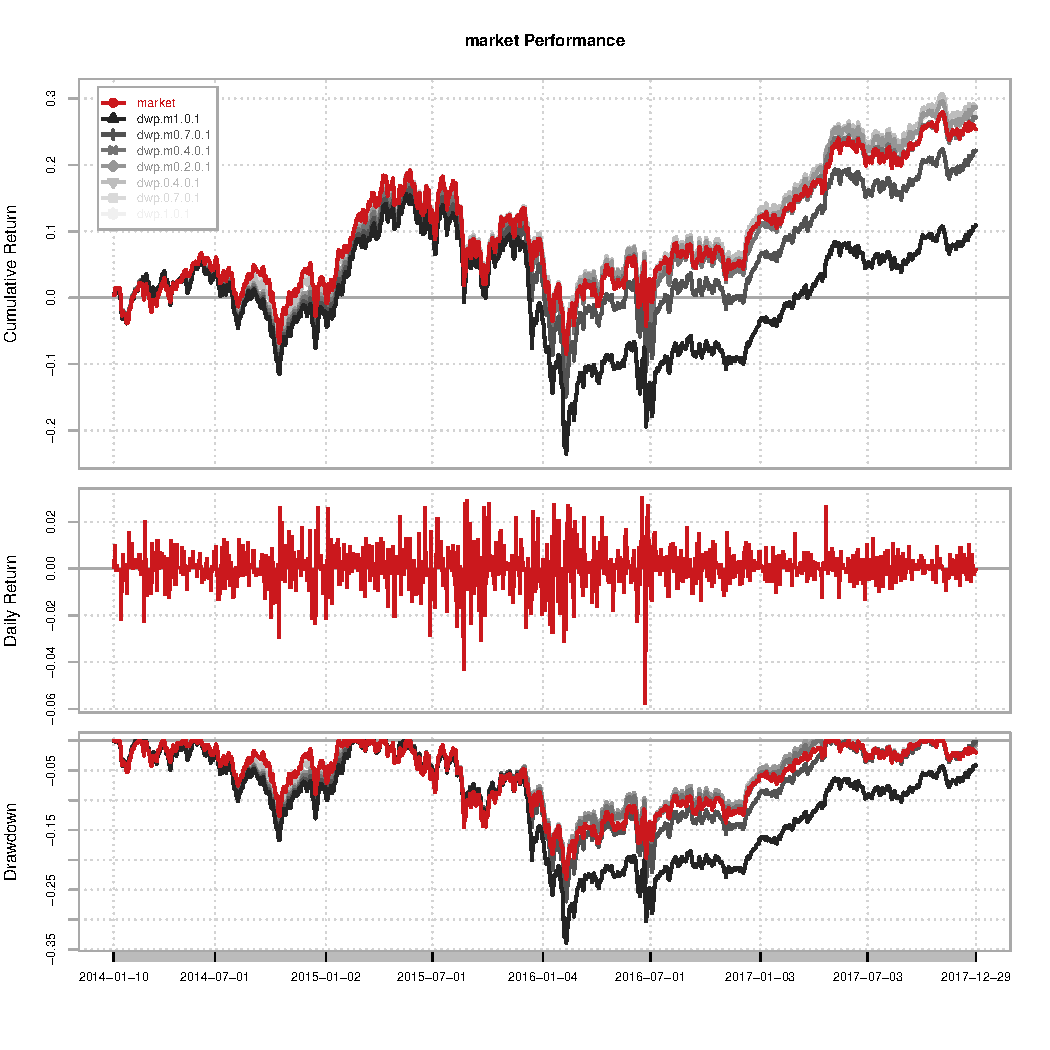
\includegraphics[width=350]{performance.pdf}

\begin{table}[!h]
  \begin{tabular}{lrrrr}
    \toprule
    \bf  & \bf 2014 & \bf 2015 & \bf 2016 & \bf 2017 \bf Annualised Return & \bf
Annualised Std Dev & Annualized Sharpe \\
    \midrule
    market & \color{red}-5.2 & 0.4 & \color{red}-0.8 & 4.9   \\
    dwp(-1.0) & \color{red}-4.4 & 1.6 & 1.2 & 4.9\\
    dwp(-0.7) & \color{red}-4.4 & 1.4 & 1.1 & 4.9\\
    dwp(-0.4) & \color{red}-4.4 & 1.2 & 0.9 & 4.9\\
    dwp(-0.2) & \color{red}-4.4 & 1.1 & 0.7 & 5.0\\
    dwp(+0.4) & \color{red}-4.7 & 0.6 & 0.0 & 5.0\\
    dwp(+0.7) & \color{red}-4.9 & 0.5 & \color{red}-0.4 & 5.0\\
    dwp(+1.0) & \color{red}-5.2 & 0.4 & \color{red}-0.8 & 4.9\\
    \bottomrule
  \end{tabular}
\end{table}

\centering
\resizebox{\linewidth}{!}{\begin{tabular}{lrrrrrrrr}
\toprule
  & market & dwp.m1.0.1 & dwp.m0.7.0.1 & dwp.m0.4.0.1 & dwp.m0.2.0.1 & dwp.0.4.0.1 & dwp.0.7.0.1 & dwp.1.0.1\\
\midrule
Semi Deviation & 0.0067 & 0.0075 & 0.0070 & 0.0069 & 0.0068 & 0.0067 & 0.0067 & 0.0067\\
Gain Deviation & 0.0060 & 0.0061 & 0.0060 & 0.0059 & 0.0059 & 0.0060 & 0.0060 & 0.0060\\
Loss Deviation & 0.0069 & 0.0083 & 0.0075 & 0.0073 & 0.0072 & 0.0071 & 0.0070 & 0.0069\\
Downside Deviation (MAR=210\%) & 0.0118 & 0.0124 & 0.0120 & 0.0118 & 0.0118 & 0.0118 & 0.0118 & 0.0118\\
Downside Deviation (Rf=0\%) & 0.0066 & 0.0074 & 0.0069 & 0.0067 & 0.0067 & 0.0066 & 0.0066 & 0.0066\\
\addlinespace
Downside Deviation (0\%) & 0.0066 & 0.0074 & 0.0069 & 0.0067 & 0.0067 & 0.0066 & 0.0066 & 0.0066\\
Maximum Drawdown & 0.2321 & 0.3392 & 0.2697 & 0.2400 & 0.2314 & 0.2281 & 0.2306 & 0.2321\\
Historical VaR (95\%) & -0.0144 & -0.0158 & -0.0153 & -0.0153 & -0.0150 & -0.0146 & -0.0146 & -0.0144\\
Historical ES (95\%) & -0.0220 & -0.0244 & -0.0227 & -0.0221 & -0.0220 & -0.0220 & -0.0220 & -0.0220\\
Modified VaR (95\%) & -0.0152 & -0.0173 & -0.0161 & -0.0157 & -0.0155 & -0.0153 & -0.0153 & -0.0152\\
Modified ES (95\%) & -0.0257 & -0.0406 & -0.0337 & -0.0315 & -0.0306 & -0.0281 & -0.0269 & -0.0257\\
\bottomrule
\end{tabular}}
\end{table}


\subsection{Simulation with Market Impact}

We extend the analysis to show how the exact same portfolios would perform if
run through a simulator that accounts for market impact using a model whos
coefficients on parameters such as volatility, average daily volume, and
turnover have been fitted on institutional trade data in a similar manner as
discussed by Almgren \cite{almgren2005direct}.

% Account for varying book sizes to see how that effects market impact
% and profitability



%%%%%%%%%%%%%%%%%%%%%%%%%%%%%%%%%%%%%%%%%%%%%%%%%%%%%%%%%%%%%%%%%%%%
\newpage
\section{Conclusion}

% TODO: Complete conclusion


%%%%%%%%%%%%%%%%%%%%%%%%%%%%%%%%%%%%%%%%%%%%%%%%%%%%%%%%%%%%%%%%%%%%
\newpage
%TODO: Ensure all theorems etc have a citation
%TODO: Ensure all references are working correctly
%TODO: Ensure formatting matches submission format
\printbibliography

\end{document}
